%% Document created 12 April 2021 automatically 
%% from /Users/massimosotgia/Desktop/uni_at_DIFI/Lab_C03/setup.py 

%% Copyright (C) Mattia Sotgia et al. 2021
%% Using class lab_unige.cls
%                                                            
%                                                            
%   **                 **             ******   ****   ****   
%  /**                /**            **////** *///** */// *  
%  /**        ******  /**           **    // /*  */*/    /*  
%  /**       ´´´´´´** /******      /**       /* * /*   ***   
%  /**        ******* /**///**     /**       /**  /*  /// *  
%  /**       **´´´´** /**  /** **  //**    **/*   /* *   /*  
%  /********//********/****** /**   //****** / **** / ****   
%  ////////  //////// /////   //     //////   ////   /´///   
%                                                            
%                                                            
\documentclass[italian, a4paper, 10pt, twocolumn]{../../style/lab_unige}
\usepackage[a4paper, margin=1.75cm, footskip=0.25in]{geometry}

\usepackage[utf8]{inputenc}
\usepackage[T1]{fontenc}

\usepackage[italian]{babel}

% \usepackage{biblatex}

\usepackage[bookmarksopen=true, citebordercolor={0 1 0}, linkbordercolor={1 0 0}, urlbordercolor={0 1 1}]{hyperref}
\usepackage[numbered]{bookmark}

\usepackage{graphicx}
\graphicspath{{../fig/}}
\usepackage{array}
\usepackage{tabulary}
\usepackage{booktabs}

% FOUNDAMENTAL
\usepackage{../../style/custom}

\usepackage{physics}

\usepackage{breqn}
\usepackage{cuted}
\usepackage{txfonts}

\usepackage{lipsum}

%% Define ref types
\newcommand{\reftab}[1]{Tabella {\ref{#1}}}%
\newcommand{\reffig}[1]{Figura {\ref{#1}}}%
\newcommand{\refeqn}[1]{({\ref{#1}})}%
%% PAPER ONLY custom Macros
\newcommand{\ChiSqr}{$\chi^2$\space}
\newcommand{\ChiNdf}{$\chi^2/\text{ndf}$}
\newcommand{\cernroot}{\texttt{root}}
\newcommand{\treSigma}{$3\sigma$}
\newcommand{\stdErr}[1]{$\varepsilon_{#1}$}
\newcommand{\mstdErr}[1]{\varepsilon_{#1}}
\newcommand{\gLab}{$g_t~=~(~9.8056~\pm~0.0001~\text{ stat}~)~\text{ m/s}^2$}


%%
\setlength{\columnsep}{6mm}

\begin{document}
    \twocolumn[
    \begin{@twocolumnfalse}
        \title{
            {\raggedright 
\includegraphics[width=0.2\linewidth]{../../style/lab_mark.pdf}\\}
            Taratura di un Dinamometro Elettronico e Verifica dell'effetto Gough-Joule \\
            Conseguenze Macroscopiche della Natura Entropica delle Forze Elastomeriche
        }
        \author{
        Eugenio Dormicchi\textsuperscript{1},
        % Riccardo Pizzimbone\textsuperscript{1}, 
        Giovanni Oliveri\textsuperscript{1},
        Mattia Sotgia\textsuperscript{1, 2}
        }

        \date{
            \textit{    
            \textsuperscript{1}Gruppo C03, Esperienza di laboratorio n. 7, \\
            \textsuperscript{2}In presenza in laboratorio per la presa dati\\
            % Università degli Studi di Genova, Dipartimento di Fisica.\\
            }
            \vspace{2ex}
            (Presa dati
            14 Aprile 2021, 15:00– 18:00; Analisi dati
            20 Aprile 2021)
        }
        \maketitle
        
        \begin{abstract}
            \textit{Obiettivo-- }
            Vogliamo costruire e tarare una bilancia elettronica che sfrutti il funzionanmento della cella di carico, e ricavare quindi una legge che permetta dei misurare la massa di un oggetto misurando la tensione in uscita dal sistema. Vogliamo poi verificare con lo strumento costruito le conseguenze macroscopiche della natura entropica delle forze elastomeriche, ovvero verificare l'effetto Gough-Joule.
            \textit{Metodi-- }
            Per la costruzione e la taratura si veda meglio la sezione dedicata. La verifica dell'effetto Gough-Joule viene effettuata aumentando la tamperatura gradualmente e misurando la tensione dell'elastomero.
            \textit{Conclusione-- }
            Non riusciamo a calibrare il dinamometro; osserviamo però un comporamento lineare sia nella relazione tra $V_0$ e $M$, che tra $f$ e $T$, dimostrando anche l'effetto Gough-Joule, almeno in forma teorica.

        \end{abstract}
        \vspace{2em}
    \end{@twocolumnfalse}
    ]

    %%%% CORPO DEL TESTO
    %%%% CORPO DEL TESTO

    \section{Obiettivo}
    \label{section:aim}

    Si vuole costruire un dinamometro il cui funzionamento è basato su una cella di carico, ed effettuarne una taratura, determinandone cioè la sua portata e la sua risoluzione. 
    Vogliamo poi utilizzare lo strumento per studiare l'effetto macroscopico che esplicita l'effetto miscroscopico legato all'entropia di un elastomero, per studiare la natura  entropica delle forze esercitate da materiali come gomme e polimeri, e i legami tra queste interazioni e le variazioni di temperatura ambientale. 

    \section{Strumentazione}
    \label{section:strument}

    Abbiamo a disposizione la seguente strumentazione:\\
    Multimetro da Banco Tektronix DMM 5-1/2 Digit Multimeter:
    Portata 1000V;
    Accuratezza dopo 1 anno a temperatura $23\pm5$ $^\circ$C : $0.0015\pm0.004$ mV;
    Risoluzione con fondo scala 200 mV in modalità slow: $1~\mu$V;
    Sensibilità che assumiamo coincidere con la risoluzione: $1~\mu$V;\\
    Generatore di tensione Agilent U8031A Triple Output DC Power Supply 0-30V, 6A/5V, 3A;\\
    Bilancia Elettronica Kern PCB-350/4, di portata 350~g, considerando come sensibilità la linearità dello strumento $40~\mu$g (non rischiamo così di sottostimare l'errore);\\
    Lab-Jack;\\
    Cella di Carico TEDEA;\\
    Termometro a bulbo di portata 150 $^\circ$C, sensibilità 1 $^\circ$C;\\
    Calibro ventesimale, di portata 0.150~m, sensibilità uguale all'accuratezza $50~\mu$m;\\
    Elastico di gomma generico;\\
    Becker graduato;\\
    Masse tarate con rispettivi valori in grammi riportati sulla scatola e in \reftab{table:masses_c};\\

    \begin{table}[h!]
        \centering
        \footnotesize
        \caption{Valori delle masse della scatola C, da 1 a 8.}
        \label{table:masses_c}
        \begin{tabular}{lr}
            \hline\hline\\[-1.5ex]
            $c_i$ &  Massa tarata [g] \\[+0.5ex] \hline \\[-1.5ex]     
            $c_1$ &  48,140           \\[+0.5ex]
            $c_2$ &  51,545           \\[+0.5ex]
            $c_3$ &  53,193           \\[+0.5ex]
            $c_4$ &  73,949           \\[+0.5ex]
            $c_5$ &  80,134           \\[+0.5ex]
            $c_6$ & 101,298           \\[+0.5ex]
            $c_7$ & 101,117           \\[+0.5ex]
            $c_8$ & 116,217           \\[+0.5ex] \hline \\[-1.5ex]
        \end{tabular}
    \end{table}

    \begin{figure}[b!]
        \centering
        \includegraphics[width=0.9\linewidth]{load_cell_full.pdf}
        \caption{\textit{In alto: } schema di costruzione di un estensimetro (strain gauge). \textit{In basso: } vista laterale della cella di carico in condizioni di riposo e in condizione di carico. Nella condizione di carico l'effetto è volutamente esagerato per illustrare la compressione di $R_1$ e $R_3$ e la estensione di $R_2$ e $R_4$.}
        \label{figure:load_cell}
    \end{figure}

    Per la prima parte dell’ esperienza, che consiste nella costruzione e  taratura di un dinamometro elettronico a cella di carico (\reffig{figure:load_cell}), si colleghi l’ alimentatore di tensione Agilent alla cella di carico facendo attenzione ad alimentarlo con tensione continua pari a 10 V. Per verificare che il valore si quello richiesto, collegare i terminali dell’ alimentatore nell’ ordine corretto al multimetro da banco. \\
    Quest’ultimo deve essere impostato sulla modalità lettura a tensione continua VDC, scegliendo il fondo scala più basso (modalità automatica). Inoltre è importante evitare che la tensione dell’ alimentatore non venga variata nel corso delle misure; a tale scopo è consigliato utilizzare il pulsante “lock”. Per selezionare il fondo scala più basso del multimetro Tecktronix e si operi in modalità slow per ottenere una maggiore risoluzione necessaria alla nostra esperienza. Come incertezza sulla lettura in tensione del multimetro, considerando il criterio della mezza divisione sull’ ultima cifra significativa, assumendo quindi incertezza pari a  $0,5~\mu$V. 

    L’ apparato sperimentale consiste infine nella cella di carico dotata di piano di appoggio, il tutto fissato con un morsetto al  rispettivo montante. Sia l’alimentatore sia il multimetro sono collegati alla scatola di connessione della cella posta sulla base del montante.

    La superficie di appoggio, che  consiste in una lastra di metallo sottile, è collocata a un estremo della cella di carico.  Le masse di cui si dispone dovranno essere posizionate sopra il piano attraverso combinazioni intelligenti fino a raggiungere una massa massima di circa 600~g (si veda anche la sezione \ref{section:methods}).

    La base del montante è fissata al tavolo da lavoro per mezzo di un secondo morsetto per impedire spostamenti indesiderati della struttura.

    La seconda parte dell’esperienza consiste nella verifica empirica dell’effetto Gough-Joule.\\
    La struttura è costituita da un piano di appoggio posto sopra la cella di carico la quale è tenuta fissa a un montante attraverso l’uso un morsetto.\\
    Un secondo morsetto fissa al banco da lavoro la base del montante che sostiene la scatola di connessione della cella di carico.
    
    Al di sotto della lastra di appoggio, perpendicolare a essa, è fissato un gancio il cui estremo inferiore giace al di sopra del becker. Quest’ultimo contiene un termometro a bulbo e un contrappeso, anche esso munito di gancio; il tutto è inserito all’ interno di un contenitore di vetro (becker) centrato sopra il Lab-Jack.\\
    Si sospende un estremo dell’ anello di elastomero al gancio della cella di carico e l’altro estremo al contrappeso che deve essere appoggiato delicatamente al fondo del becker.\\
    Si abbassi il piano del Lab-Jack in modo da allungare l’elastico di una lunghezza circa pari a due volte la lunghezza di riposo portando il gancio all’orlo del becker. 
    
    \section{Metodi}
    \label{section:methods}

    Tutte le misure sono riportate nelle unità del Sistema Internazionale (SI), nel caso della tensione, si è utilizzato un sottomultiplo per evitare di rendere i calcoli difficili.\\
    I valori riportati sono stati approssimati tenendo conto di alcune convenzioni prese. Si approssima l'errore a una cifra significativa se tale cifra è $\geqslant3$, altrimenti se tale cifra è 1 o 2 allora si considerano due cifre significative. Considerando quindi le posizioni decimali significative dell'errore si approssima per eccesso il valore numerico della grandezza.\\
    Si fa spesso riferimento anche alla regola del \treSigma, con la quale si vuole intendere la volontà di trasformare un errore di tipo massimo in errore statistico, ovvero calcolando $\mstdErr{x}~=~\Delta x/\sqrt{3}$.\\

    \subsection{Taratura dinamometro sperimentale}

    La cella di carico utilizzata, mostrata in \reffig{figure:load_cell}, presenta quattro estensimetri (straing gauge) che rappresentano le resistenze $R_1$, $R_2$, $R_3$, e $R_4$, i quali subiscono estensione o compressione quando il carico viene applicato sulla cella. Quando subiscono compressione o estensione la loro resistenza diminuisce (compressione) o aumenta (estensione). Posta la cella di carico come in \reffig{figure:load_cell} in basso, $R_1$ e $R_3$ risultano avere resistenza maggiore, mentre $R_2$ e $R_4$ risultano avere resistenza minore. se consideriamo $\varepsilon=\Delta L/L$ la variazione di lunghezza dell'estensimetro, otteniamo che $\Delta R/R = k\varepsilon$ dove $k$ è un fattore di proporzionalità (gauge factor). Se consideriamo un’approssimazione di piccoli carichi $F$, allora $\varepsilon$ è proporzionale al carico applicato, $\varepsilon=cF$.\\
    La variazione di resistenza può essere misurata in vari modi, ma è una variazione che corrisponde circa allo $0.1\%/0.01\%$. Sfruttiamo perciò lo schema di misura a ponte di Wheatstone, come rappresentato in \reffig{figure:multimeter_ps}, che trasforma variazioni di misura di resistenze in variazioni ben più evidenti di tensioni, lette poi dal multimetro come $V_0$.

    \begin{figure}
        \centering
        \includegraphics[width=0.9\linewidth]{multimeter_ps_full.pdf}
        \caption{\textit{In alto:} multimetro da banco Tektronix DMM 5-1/2 Digit Multimeter impostato su scala automatica, modalità \texttt{Slow} che consente una lettura più precisa della tensione; generatore di corrente DC Agilent U8031A Triple Output DC Power Supply, con una tensione in uscita sull'output-1 di 10.00 V. \textit{In basso:} Schema elettrico del ponte di Wheatstone utilizzato per amplificare la variazione delle resistenze. $V_0$ indica la tensione misurata con il multimetro, mentre $V_S$ indica la tensione erogata dal generatore che alimenta tale ponte.}
        \label{figure:multimeter_ps}
    \end{figure}

    In assenza di carico le resistenze sono nulle, e la tensione in uscita è $V_0=0V$, in presenza di carico invece la tensione è legata alla forza esercitata come
    \begin{equation}
        V_0=V_sk\varepsilon=V_skcF\text{ ($V_s=10.00V$).}\label{equation:v0_f}
    \end{equation}
    
    
    In realtà la cella di carico stessa presenta una massa, oltre che dover sostenere il piatto su cui verranno successivamente posate le masse per la taratura, e quindi anche in condizione di riposo il multimetro segna una tensione~$\neq0$, 
    \[V_{\text{scarico}}=0.845\text{ mV.}\]

    Per tarare il dinamometro sperimentale creato prendiamo in considerazione otto corpi di massa nota senza errore \reftab{table:masses_c}, e li combiniamo in modo da ottenere 15 valori (da circa $5.0\times10^{-2}$~kg fino a $5.50\times10^{-1}$~kg) di masse. Queste masse vengono poi posate sul piatto della cella di carico e ne viene misurata la tensione $V_0$ dal ponte di Wheatstone. È importante mantenere il carico della cella inferiore ai 600~g, in quanto una massa superiore porterebbe allo snervamento del metallo e rovinerebbe in modo permanente lo strumento. 
    Se ora partendo dalla equazione \ref{equation:v0_f} consideriamo la forza come forza peso ricaviamo ($F=Mg$)
    \begin{equation}
        V_0=V_sk\varepsilon=V_skcgM\text{ ($V_s=10.00$~V).}\label{eqation:v0_mg}
    \end{equation}

    \begin{table}
    \footnotesize
    \centering
    \caption{Dati prima parte, taratura strumento.}
    \label{table:p1}
    \begin{tabular}{ccl}
        \hline\hline\\[-1.5ex]
        Tensione [mV]       & \multicolumn{2}{c}{Massa [kg]}                         \\[+0.5ex]
        $V_{0,~i}(\pm\mstdErr{V_0})$ & $m_i$      &  (Combinazioni)                  \\[+0.5ex] \hline \\[-1.5ex]
        $ 2.199(\pm0.0003)$          & $0.048140$ &  ($c_1$)                         \\[+0.5ex]
        $ 2.926(\pm0.0003)$          & $0.073949$ &  ($c_4$)                         \\[+0.5ex]
        $ 3.649(\pm0.0003)$          & $0.099685$ &  ($c_1+c_2$)                     \\[+0.5ex]
        $ 4.112(\pm0.0003)$          & $0.116217$ &  ($c_8$)                         \\[+0.5ex]
        $ 5.145(\pm0.0003)$          & $0.152843$ &  ($c_2+c_6$)                     \\[+0.5ex]
        $ 5.769(\pm0.0003)$          & $0.175066$ &  ($c_4+c_7$)                     \\[+0.5ex]
        $ 6.539(\pm0.0003)$          & $0.202415$ &  ($c_6+c_7$)                     \\[+0.5ex]
        $ 7.989(\pm0.0003)$          & $0.253960$ &  ($c_2+c_6+c_7$)                 \\[+0.5ex]
        $ 8.619(\pm0.0003)$          & $0.276364$ &  ($c_4+c_6+c_7$)                 \\[+0.5ex]
        $ 9.808(\pm0.0003)$          & $0.318632$ &  ($c_6+c_7+c_8$)                 \\[+0.5ex]
        $11.161(\pm0.0003)$          & $0.366772$ &  ($c_1+c_6+c_7+c_8$)             \\[+0.5ex]
        $12.061(\pm0.0003)$          & $0.398766$ &  ($c_5+c_6+c_7+c_8$)             \\[+0.5ex]
        $14.141(\pm0.0003)$          & $0.472715$ &  ($c_4+c_5+c_6+c_7+c_8$)         \\[+0.5ex]
        $15.637(\pm0.0003)$          & $0.525908$ &  ($c_3+c_4+c_5+c_6+c_7+c_8$)     \\[+0.5ex]
        $17.087(\pm0.0003)$          & $0.577453$ &  ($c_2+c_3+c_4+c_5+c_6+c_7+c_8$) \\[+0.5ex] \hline \\[-1.5ex]
    \end{tabular}
\end{table}

    Considerando il termine $V_skcg$ costante possiamo descrivere una relazione lineare $V=aM$, in cui introduciamo anche un fattore correttivo $b$ per giustificare il fatto che con $M=0$, e quindi con la cella scarica, $V_{\text{scarico}}\neq0$. La legge diventa quindi
    \begin{equation}
        V_0=aM+b\label{equation:v0_m}
    \end{equation}
    Misurati i valori di $V_0$ per ognuna delle 15 masse riportiamo i valori in \reftab{table:p1}, e associamo ai valori di $V_0$ un errore statistico ricavato dalla mezza misura della sensibilità dello strumento, staticizzata dividendo ulteriormente per $\sqrt{3}$, ottenendo quindi \[\mstdErr{V_0} = 0.001/(2\cdot\sqrt{3})=0.0003\text{ mV.}\]

    Inoltre abbiamo verificato con un piccolo filo di rame di lunghezza circa 7~mm quale fosse la massa più piccola che faceva scartare di 0.001~mV il multimetro collegato alla cella di carico. abbiamo quindi misurato con la bilancia elettronica il valore della sua massa, ottenendo $m_{\text{min}}^s=(0.034\pm0.002\text{ stat})$~g.

    \subsection{Misura di $\Delta V$ in relazione alla temperatura}

    Per verificare sperimentalmente l'effetto Gough-Joule si utilizza una sua conseguenza macroscopica. È noto che in un solido sottoposto ad un aumento di temperatura i legami interni si indeboliscano, come si può osservare in un metallo. Il comportamento degli elastomeri è invece contro-intuitivo e in particolare si osserva una contrazione del solido all'aumentare della temperatura. Questo comportamento è legato alla natura entropica dell'elastomero; la gomma in particolar modo quando viene scaldata aumenta la sua entropia interna, e quindi i singoli filamenti interni si dispongono in modo caotico, facendo contrarre il solido. \\
    In un elastomero, il maggior effetto che si può osservare quando un carico viene applicato è l'allineamento delle catene polimeriche e quindi un allineamento dei monomeri. In questo modo si ha una riduzione dell'entropia. Se il corpo viene invece rilasciato, il sistema tornerebbe a uno stato a entropia maggiore, per cui il corpo complessivamente si accorcerebbe. In modo analogo, se forniamo calore a un elastomero allungato, aumentiamo l'entropia del sistema, che corrisponde a una tendenza delle catene polimeriche a ritornare in uno stato caotico, quindi accorciamo macroscopicamente il solido; togliendo calore invece allunghiamo il corpo, che ritorna a uno stato a entropia minore.\\
    Vogliamo sfruttare il dinamometro creato e tarato per verificare sperimentalmente questo comportamento.\\
    Si può dimostrare che la tensione $f$ esercitata da un elastomero allungato fino a $l$ da $l_0$ è con buona approssimazione
    \begin{equation}
        f=\frac{NK_BT}{l_0}\left(\alpha-\alpha^{-2}\right)\label{equation:f_T}
    \end{equation}
    con $N$ il numero di catene monomeriche dell'elastico, $K_B=1.3806\times10^{-23}$~J/K è la costante di Boltzmann, $T$ la temperatura in kelvin, $l_0$ la lunghezza a riposo dell'elastico e $\alpha$ l'elongazione relativa, definita come $\alpha=\frac{l}{l_{0}}$. Con $\alpha$ costante possiamo osservare una relazione lineare tra $f$ e $T$.
    
    
    Innanzitutto con un calibro misuriamo la lunghezza interna dell'elastico, $l_{0}\approx29$~mm. Su il gancio fissato sulla cella di carico colleghiamo un capo dell'elastico, l'altro lo attacchiamo al gancio sul contrappeso posto in fondo al becker posto sul Lab-Jack, che regoliamo in modo da avere una lunghezza tra i due ganci $l\approx2\cdot l_{0}\approx58$~mm. Ricaviamo l'elongazione relativa $\alpha=\frac{l}{l_{0}}=\frac{2\cdot l_0}{l_0}=2$.\\
    Riempito il becker con acqua calda ($T_K=58$~K), quando il termometro segna una temperatura stabile e non in discesa o in salita, facciamo partire un cronometro e misuriamo dopo 30~s, 1~min, 2~min e 3~min il valore di $V_0$ letto dal multimetro, riportiamo tutti i valori in \reftab{table:p2}.
    
    
    Abbassiamo la temperatura aggiungendo acqua fredda, scalando $T$ a intervalli di circa 5 $^\circ$C, fino a raggiungere circa 20 $^\circ$C, oltre quale troviamo difficile scendere, pur continuando ad aggiungere acqua fredda. Per ogni $T$ attendiamo che sia stabile e poi azioniamo il cronometro, ripetendo la misura dopo 30~s/1~min/2~min/3~min.\\
    Infine proviamo ad aumentare da 20 $^\circ$C la temperatura a intervalli di circa 10~K, raggiungendo il valore di circa 49 $^\circ$C. Tuttavia le tensioni misurate a queste temperature sono molto incerte, perché le temperature non sono stabili, e tendono a scendere, probabilmente a causa del contrappeso di metallo posto sul fondo del becker che rallenta il processo di riscaldamento dell'acqua, disperdendo molto del calore immerso. Infatti per le tre misure effettuate osserviamo che la temperatura nell'arco dei tre minuti della misurazione tende a scendere di circa 4-6~K.
    
    Durante lo svolgimento dell’esperienza si faccia attenzione ad non urtare il sistema per non introdurre errori sistematici.

    \section{Analisi dati}
    \label{section:analysis}

    \subsection{Taratura dinamometro}

    \begin{figure}
        \centering
        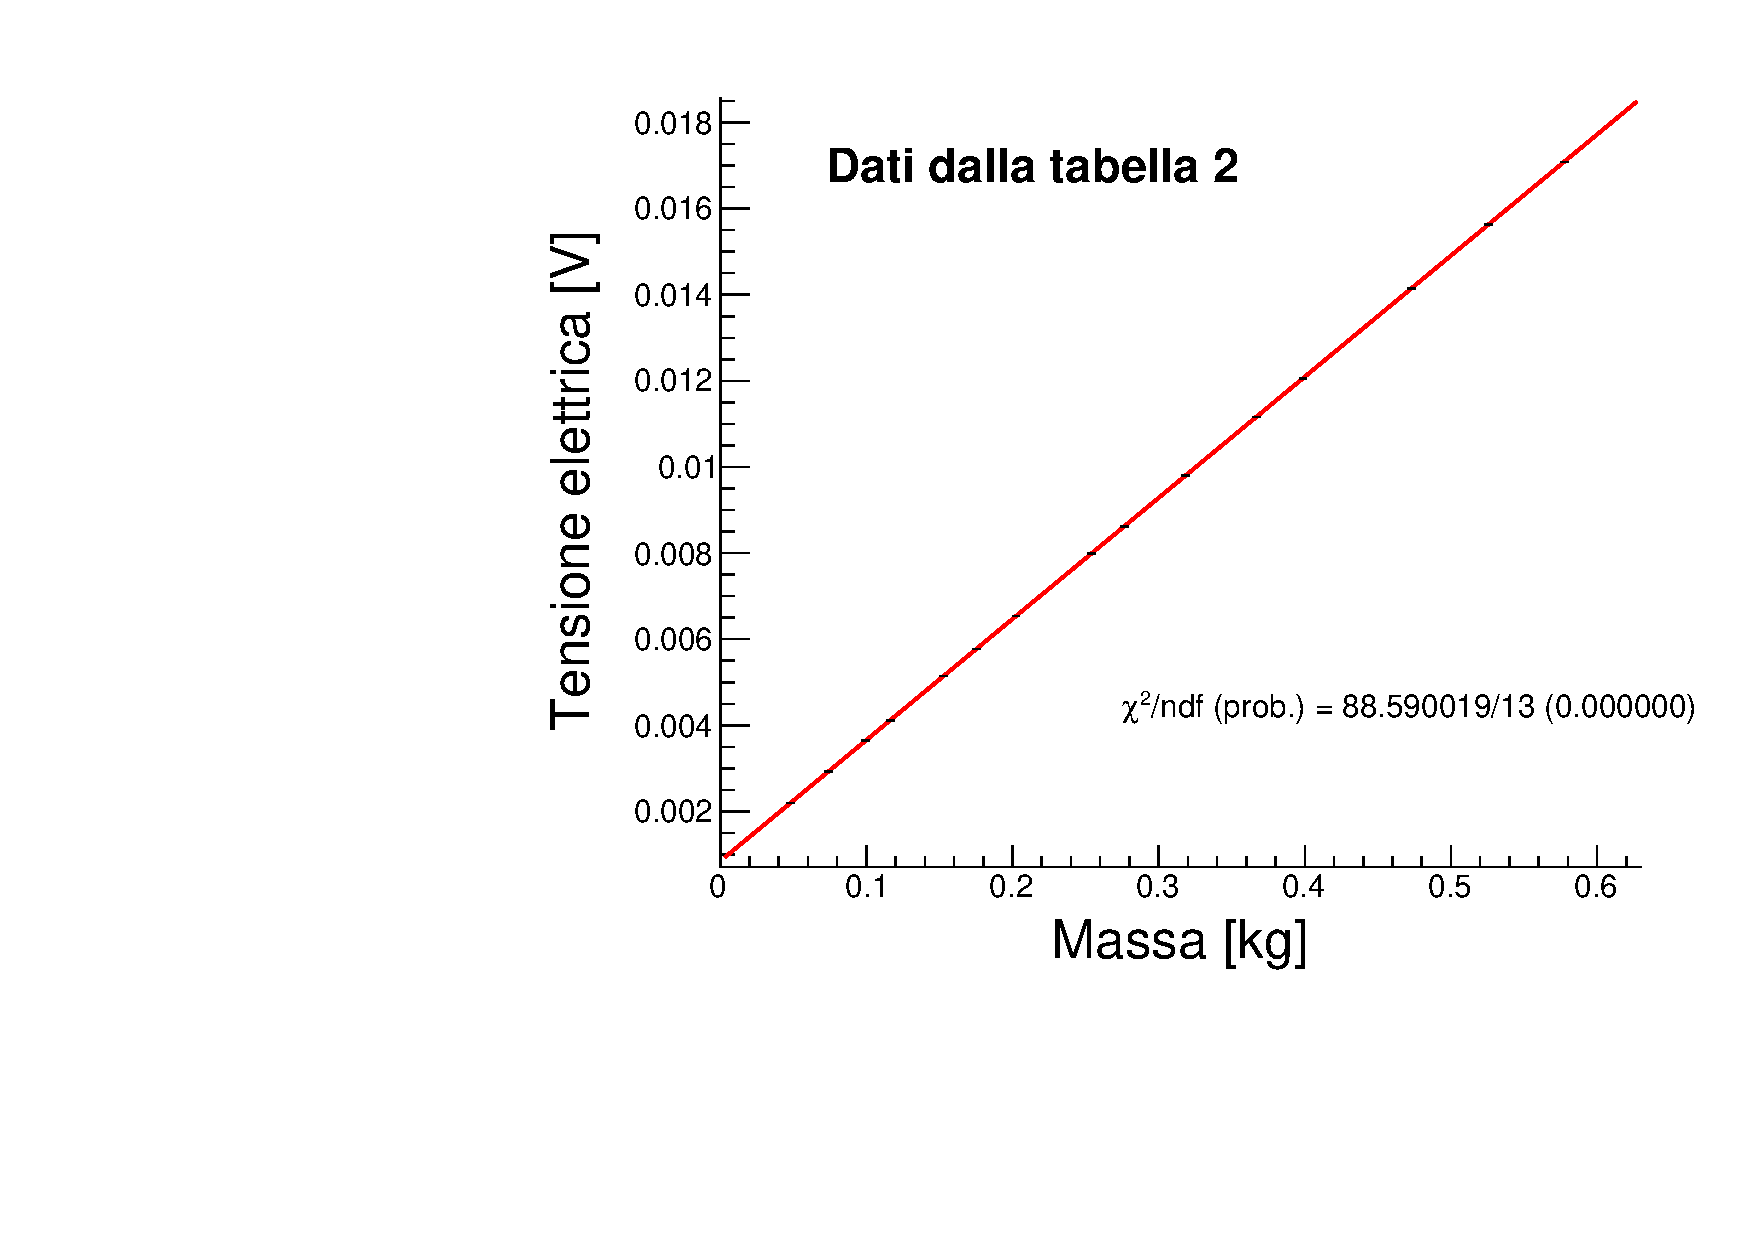
\includegraphics[width=\linewidth]{tar_plot.pdf}
        \caption{Grafico dell tensione elettrica $V_0$ in funzione della massa $M$.}
        \label{figure:tar_plot}
    \end{figure}

    Riportiamo i valori di $V_0$ in funzione di $M$ ed effettuiamo un fit lineare, per mezzo di \cernroot, secondo la legge lineare $V_0=aM+b$ (\reffig{figure:tar_plot}).\\
    L’obiettivo è quello di trovare il limite del regime di linearità del dinamometro e quindi la sua portata.\\
    Operativamente procediamo eliminando una massa per volta dal Fit, partendo dalla massa maggiore, fino a ottenere un valore del rapporto \ChiNdf~ circa equivalente a 1, e un valore della probabilità del \ChiSqr circa superiore 5-10\%.\\
    Tuttavia dal nostro Fit notiamo che il \ChiSqr è molto elevato (\ChiSqr$=88.59$) e non diminuisce in modo apprezzabile eliminando le ultime masse, di conseguenza procediamo mantenendo tutte e 15 i valori misurati. Questo non ci permette di concludere nulla di quantitativamente concreto sulla portata del nostro dinamometro.

    Otteniamo però dal Fit i valori dei parametri $a=2.81266\pm0.00005\times10^{-2}$~kg/V e $b=(0.8453\pm0.0014)$~mV, che ci permettono di costruire la relazione 
    \[
        M = \frac{V_0-b}{a}  
    \]
    da cui possiamo ricavare il valore di una qualsiasi massa conoscendo la tensione $V_0$ in uscita.

    Per individuare la sensibilità del dinamometro costruito prendiamo in considerazione la minima variazione misurabile dal voltmetro (0.001~mV) e considerando la seguente relazione \[M_{\text{min}}^t = \frac{V_{0,~\text{min}}}{a}\] otteniamo $M_{\text{min}}^t=(0.0356\pm0.0006)$~g.

    \subsection{Analisi dell'effetto di contrazione termica}
    
    \begin{table}
    \footnotesize
    \centering
    \caption{Tensione al variare della temperatura. Sono stati presi quattro valori della tensione a 30~s, 1~min, 2~min e 3~min dal momento in cui la temperatura del liquido era stabile, poiché per alcuni fenomeni di isteresi dell'elastomero la contrazione presenta un effetto di deriva, e quindi risulta importante effettuare una misura rispetto al tempo. Nel prendere il valore della tensione riportiamo tra parentesi le cifre che scalavano più velocemente, che consideriamo come incertezza massima. Le ultime tre righe riportano valori di tensione a temperature in salita, però osserviamo che le tre temperature (segnate con *) risultano essere estremamente instabili, e tendono a decrescere molto velocemente, perdendo circa 4-6~K in 3~min.}
    \label{table:p2}
    \begin{tabular}{ccccc}
        \hline\hline\\[-1.5ex]
        \multicolumn{4}{c}{Tensione $V_0$ [mV]} & Temperatura $T_i^{(k)}$ [K] \\[+0.5ex]
        a 30~s  & a 1~min & a 2~min & a 3~min   & $273.15+T_i^{\text{(deg)}}$ \\[+0.5ex] \hline \\[-1.5ex]
        7.7(50) & 7.7(21) & 7.7(00) & 7.6(61)   & $273.15+58$                 \\[+0.5ex]
        7.5(93) & 7.5(85) & 7.5(63) & 7.54(6)   & $273.15+54$                 \\[+0.5ex]
        7.4(95) & 7.4(87) & 7.47(3) & 7.46(0)   & $273.15+50$                 \\[+0.5ex]
        7.3(88) & 7.38(3) & 7.37(4) & 7.36(3)   & $273.15+45$                 \\[+0.5ex]
        7.30(4) & 7.30(1) & 7.29(5) & 7.28(8)   & $273.15+40$                 \\[+0.5ex]
        7.21(3) & 7.21(0) & 7.20(6) & 7.20(0)   & $273.15+35$                 \\[+0.5ex]
        7.14(3) & 7.14(0) & 7.14(0) & 7.13(5)   & $273.15+30$                 \\[+0.5ex]
        7.03(3) & 7.03(1) & 7.03(1) & 7.02(8)   & $273.15+25$                 \\[+0.5ex]
        6.97(6) & 6.97(6) & 6.97(6) & 6.97(7)   & $273.15+20$                 \\[+0.5ex] \hline \\[-1.5ex]
        7.10(6) & 7.10(4) & 7.10(0) & 7.09(6)   & $273.15+30^*$               \\[+0.5ex]
        7.22(1) & 7.21(9) & 7.21(5) & 7.21(1)   & $273.15+39^*$               \\[+0.5ex]
        7.37(8) & 7.37(5) & 7.36(5) & 7.35(8)   & $273.15+49^*$               \\[+0.5ex] \hline \\[-1.5ex]
    \end{tabular}
\end{table}

    Sfruttando il dinamometro costruito otteniamo i valori di tensione rispetto alla variazione di temperatura riportati in \reftab{table:p2}.

    Per verificare la legge lineare mostrata nella relazione \ref{equation:f_T} dobbiamo ottenere i valori di $f$. Sfruttiamo quindi la legge \ref{equation:v0_m}, sapendo che se $f=Mg$ allora $M=\frac{f}{g}$, conoscendo \gLab, possiamo ottenere \[f=\left(\frac{V_0-b}{a}\right)g=\left(\frac{V_0-V_{0,~0}}{a}\right)g,\] dove $b$ è $V_{0,~0}=(0.8570\pm0.0003)$~mV il valore della tensione ottenuto ponendo l'elastico appeso alla struttura nella posizione di equilibrio per valutare gli efffetti della forza di Archimede, con il relativo errore associato \[\mstdErr{f}=\sqrt{\left(\frac{g}{a}\right)^2\mstdErr{V_0}^2+\left(-\frac{g}{a}\right)^2\mstdErr{V_{0,~0}}^2+\left(-\frac{V_0-V_{0,~0}}{a^2}g\right)^2\mstdErr{a}^2}.\]

    Trascriviamo i valori così ottenuti in \reftab{table:p2a}, ed eseguiamo un grafico per i valori di $f$ rispetto a $T$ presi ai rispettivi tempi. 

    \begin{figure}
        \centering
        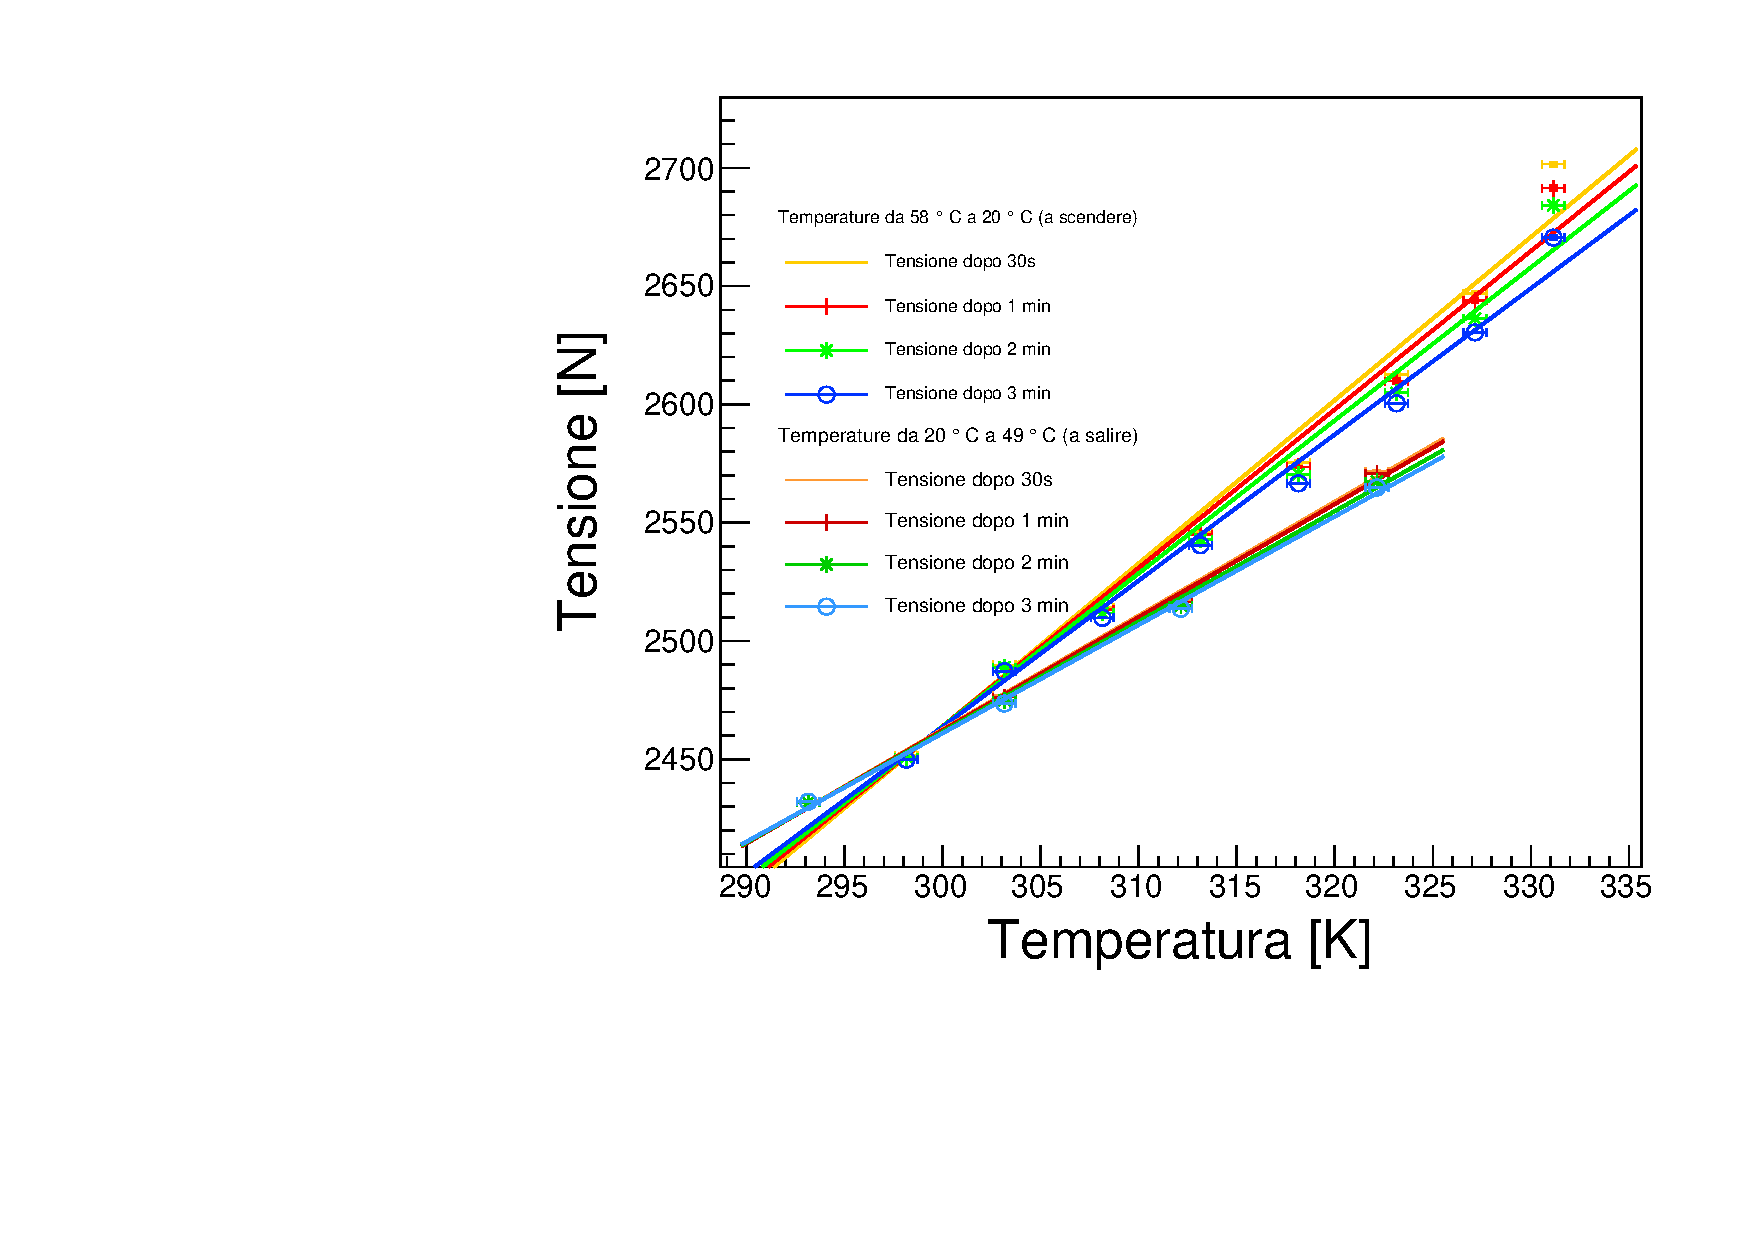
\includegraphics[width=\linewidth]{plot_istresi.pdf}
        \caption{Grafico di $f$ in funzione di $T$.}
        \label{figure:plot_isteresi}
    \end{figure}

    Possiamo ora eseguire un Fit lineare con legge \ref{equation:f_T} dove il termine $NK_B(\alpha-\alpha^{-2})/l_0$ può essere considerato costante. Lo poniamo uguale quindi a $k$ e otteniamo $f=kT$.\\
    Dal Fit possiamo quindi ottenere il valore di $k\pm\mstdErr{k}$, e infine ricavare il numero $N$ di monomeri che sono presenti nell'elastomero\[k=\frac{NK_B}{l_0}\left(\alpha-\alpha^{-2}\right),\] da cui otteniamo \[N=\frac{kl_0}{K_B\left(\alpha-\alpha^{-2}\right)}\] e il relativo errore statistico \[\mstdErr{N}=\sqrt{\left(\frac{k}{K_B\left(\alpha-\alpha^{-2}\right)}\right)^2\mstdErr{l_0}^2+\left(\frac{l_0}{K_B\left(\alpha-\alpha^{-2}\right)}\right)^2\mstdErr{k}^2}.\]

    \section{Risultati}
    \label{section:results}

    Dalla analisi dati otteniamo che per quanto riguarda la taratura dello strumento non riusciamo a determinare la portata, ma siamo riusciti a determinarne la sensibilità ($M_{\text{min}}^t = (0.0356\pm0.0006)$~g).

    Dall'analisi dati dell'effetto Gough-Joule possiamo invece ottenere valori di $N$, come mostrato nel listato in appendice \ref{section:ext}, che sono tutti dell'ordine di grandezza di $10^{22}$.

    \section{Conclusione}
    \label{section:conclusion}

    \subsection{Controlli e Possibili errori sistematici}

    Nella prima parte dell’esperienza, in seguito all’ esecuzione del fit  del grafico della relazione tra la  massa applicata al dinamometro e il voltaggio rilevato dal multimetro, abbiamo osservato un alto rapporto tra il \ChiSqr e i gradi di libertà (ndf). Pur omettendo uno, due, o più dati a partire dai più elevati, il rapporto tra i due valori rimane costantemente alto (e la probabilità del \ChiSqr rimane molto inferiore al 5-10\%). Supponiamo che la causa di questo fatto possa essere un errore sistematico dovuto allo snervamento della cella di carico utilizzata nel corso dell’esperienza, evento che non può però essere ora verificato.

    Nonostante questo osserviamo che il valore di $b$ è compatibile con quello di $V_{\text{scarico}}=0.845\text{ mV.}$, segnando comunque una certa attendibilità dei valori dei parametri $a$ e $b$ ottenuti.

    Inoltre la sensibilità teorica dello strumento è compatibile con la sensbilità sperimentare misurata ($M_{\text{min}}^t = (0.0356\pm0.0006)$~g è compatibile con $m_{\text{min}}^s=(0.034\pm0.002)$~g).

    Nell'osservare il grafico in \reffig{figure:plot_isteresi} possiamo notare che nei tre grafici ottenuti con le temperature in salita il grafico blu a occhio è il più lineare, cosa che è confermata anche dal rapporto \ChiNdf$=38.4733 / 7$, il più alto dei quattro casi. Probabilmente rimuovendo il primo punto a destra otterremmo anche un rapporto \ChiNdf~ più basso; purtroppo per mancanza di tempo non siamo riusciti a eseguire questa prova.\\
    Quindi il valore più attendibile di $N$ da questi dati è circa $N = 7.41\pm0.27$~catene monomeriche.

    Osservando invece i valori ottenuti facendo risalire la temperatura osserviamo che i punti sono tutti molto vicini ai grafici, cosa che è sottolineata dei rapporti \ChiNdf$\approx1$. Inoltre sono tutti dell'ordine di grandezza circa di $10^{22}$, che corrisponde alle aspettative.


    \appendix

    % \setcounter{table}{0}
    % \renewcommand{\thetable}{A\arabic{table}}

    \section{Dati estesi}
    \label{section:ext}

    Aggiungiamo di seguito il listato di output di \cernroot, utilizzato nell versione \verb|6.22/06|.
    {\fontsize{6}{6}
\begin{verbatim}
 **********
    RUN 0, PROCESSING 15 POINTS...
 **********

 FCN=88.59 FROM MINOS     STATUS=SUCCESSFUL     12 CALLS          78 TOTAL
                     EDM=2.88123e-17    STRATEGY= 1      ERROR MATRIX ACCURATE 
  EXT PARAMETER                                   STEP         FIRST   
  NO.   NAME      VALUE            ERROR          SIZE      DERIVATIVE 
   1  p0           8.45297e-04   1.44609e-07   6.42644e-13  -2.67559e-02
   2  p1           2.81266e-02   4.57961e-07   4.57961e-07  -7.30571e-01

** CHI2 / NDF ( PROB. ) 88.59 / 13 ( 2.59857e-13 )


 **********
    READING FROM INPUT ../dati/effetto_G_J_Tdown.txt
 **********


 **********
    PROCESSING G30...
 **********

 FCN=72.3069 FROM MINOS     STATUS=SUCCESSFUL     62 CALLS         254 TOTAL
                     EDM=2.18658e-08    STRATEGY= 1      ERROR MATRIX ACCURATE 
  EXT PARAMETER                                   STEP         FIRST   
  NO.   NAME      VALUE            ERROR          SIZE      DERIVATIVE 
   1  p0           3.95020e+02   1.57411e+01  -9.07982e-01   8.66647e-04
   2  p1           6.89614e+00   5.03366e-02   5.03366e-02   2.42091e-01

** CHI2 / NDF ( PROB. ) 72.3069 / 7 ( 5.04393e-13 )


 **********
    PROCESSING G1...
 **********

 FCN=55.7073 FROM MINOS     STATUS=SUCCESSFUL     45 CALLS         216 TOTAL
                     EDM=2.9432e-07    STRATEGY= 1      ERROR MATRIX ACCURATE 
  EXT PARAMETER                                   STEP         FIRST   
  NO.   NAME      VALUE            ERROR          SIZE      DERIVATIVE 
   1  p0           4.55748e+02   4.52419e+01   1.60774e-01   2.98080e-05
   2  p1           6.69415e+00   1.44687e-01   1.44687e-01  -4.21615e-04

** CHI2 / NDF ( PROB. ) 55.7073 / 7 ( 1.07953e-09 )


 **********
    PROCESSING G2...
 **********

 FCN=54.1923 FROM MINOS     STATUS=SUCCESSFUL     68 CALLS         261 TOTAL
                     EDM=3.72206e-11    STRATEGY= 1      ERROR MATRIX ACCURATE 
  EXT PARAMETER                                   STEP         FIRST   
  NO.   NAME      VALUE            ERROR          SIZE      DERIVATIVE 
   1  p0           5.24201e+02   1.36875e+01  -3.65367e-03  -4.84735e-08
   2  p1           6.46572e+00   4.37562e-02   4.37562e-02   9.42328e-01

** CHI2 / NDF ( PROB. ) 54.1923 / 7 ( 2.1546e-09 )


 **********
    PROCESSING G3...
 **********

 FCN=38.4733 FROM MINOS     STATUS=SUCCESSFUL     44 CALLS         212 TOTAL
                     EDM=2.67048e-07    STRATEGY= 1      ERROR MATRIX ACCURATE 
  EXT PARAMETER                                   STEP         FIRST   
  NO.   NAME      VALUE            ERROR          SIZE      DERIVATIVE 
   1  p0           6.10696e+02   1.87998e+01  -2.06160e-01   6.42299e-05
   2  p1           6.17684e+00   6.00758e-02   6.00758e-02   2.09922e-02

** CHI2 / NDF ( PROB. ) 38.4733 / 7 ( 2.46268e-06 )


 **********
    RISULTATI PER TEMPERATURE A SCENDERE PER N
 **********

N (da V_0 a 30 s)  = 8.27749e+21 +/- 2.91755e+20
N (da V_0 a 1 min) = 8.03503e+21 +/- 3.27e+20
N (da V_0 a 2 min) = 7.76085e+21 +/- 2.7272e+20
N (da V_0 a 3 min) = 7.4141e+21 +/- 2.65633e+20

 **********
    READING FROM INPUT ../dati/effetto_G_J_Tup.txt
 **********


 **********
    PROCESSING G30_UP...
 **********

 FCN=1.85026 FROM MINOS     STATUS=SUCCESSFUL     67 CALLS         289 TOTAL
                     EDM=1.04287e-09    STRATEGY= 1      ERR MATRIX NOT POS-DEF
  EXT PARAMETER                APPROXIMATE        STEP         FIRST   
  NO.   NAME      VALUE            ERROR          SIZE      DERIVATIVE 
   1  p0           9.54309e+02   2.65238e+01  -5.34615e-02  -4.58570e-08
   2  p1           5.01687e+00   8.47162e-02   8.47162e-02  -4.42370e-03

** CHI2 / NDF ( PROB. ) 1.85026 / 1 ( 0.173754 )


 **********
    PROCESSING G1_UP...
 **********

 FCN=1.73906 FROM MINOS     STATUS=SUCCESSFUL     61 CALLS         247 TOTAL
                     EDM=1.69866e-09    STRATEGY= 1      ERROR MATRIX ACCURATE 
  EXT PARAMETER                                   STEP         FIRST   
  NO.   NAME      VALUE            ERROR          SIZE      DERIVATIVE 
   1  p0           9.59665e+02   3.44815e+01   4.32344e-01   1.98619e-04
   2  p1           4.99712e+00   1.10325e-01   1.10325e-01   2.60379e-02

** CHI2 / NDF ( PROB. ) 1.73906 / 1 ( 0.187258 )


 **********
    PROCESSING G2_UP...
 **********

 FCN=1.12949 FROM MINOS     STATUS=SUCCESSFUL     67 CALLS         283 TOTAL
                     EDM=2.37203e-09    STRATEGY= 1      ERR MATRIX NOT POS-DEF
  EXT PARAMETER                APPROXIMATE        STEP         FIRST   
  NO.   NAME      VALUE            ERROR          SIZE      DERIVATIVE 
   1  p0           9.94378e+02   2.57764e+01  -5.13522e-02  -1.48168e-12
   2  p1           4.87934e+00   8.24237e-02   8.24237e-02  -8.16232e-03

** CHI2 / NDF ( PROB. ) 1.12949 / 1 ( 0.287884 )


 **********
    PROCESSING G3_UP...
 **********

 FCN=0.865242 FROM MINOS     STATUS=SUCCESSFUL     38 CALLS         195 TOTAL
                     EDM=1.29983e-08    STRATEGY= 1      ERROR MATRIX ACCURATE 
  EXT PARAMETER                                   STEP         FIRST   
  NO.   NAME      VALUE            ERROR          SIZE      DERIVATIVE 
   1  p0           1.01089e+03   7.02799e+01   3.22983e-01   1.20934e-04
   2  p1           4.82091e+00   2.24823e-01   2.24823e-01  -3.66225e-03

** CHI2 / NDF ( PROB. ) 0.865242 / 1 ( 0.352276 )


 **********
    RISULTATI PER TEMPERATURE A SALIRE PER N
 **********

N (da V_0 a 30 s)  = 6.02177e+21 +/- 2.31208e+20
N (da V_0 a 1 min) = 5.99808e+21 +/- 2.45591e+20
N (da V_0 a 2 min) = 5.8567e+21 +/- 2.24886e+20
N (da V_0 a 3 min) = 5.78657e+21 +/- 3.35615e+20
\end{verbatim}}
    

\end{document}
    
